\chapter{Implementation Broker}

\section{Protocol implementation}
\label{sec-protocol}
\subsection{Primitive Types}
All messages are size delimited and are made up of the following primitive
types: 

\begin{table}[h]
\begin{tabular}{| p{3cm}| p{7cm} | l |}
\hline
\textbf{Type} & \textbf{Description} & \textbf{Variations} \\ \hline
Fixed Width Primitives     & Signed integers stored in big endian order.                                                                                                                                     & int8, int16, int32, int64 \\ \hline
Variable Length Primitives & Consist of a signed integer giving a length N followed by N bytes of content. A length of -1 indicates null. String uses an int16 for its size, and bytes uses an int32.        & bytes, string             \\ \hline
Arrays                     & Repeated structures. Always be encoded as an int32 size containing the length N followed by N,repetitions of the structure which can itself be made up of other,primitive types &                           \\ \hline
\end{tabular}
\end{table}

\subsection{Common Message Format}
The message as unit of transported data has the following common structure of a
message set which is used for all api's which transport message data.
Furthermore this format happens to be used both for the on-disk storage on the
broker and the on-the-wire format.

\begin{figure}[H]
    \centering
    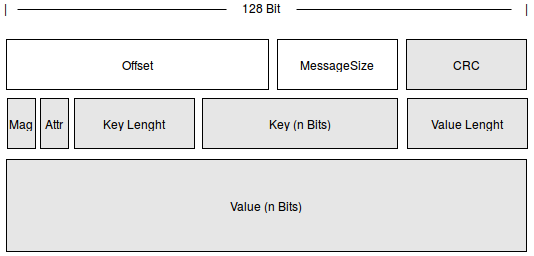
\includegraphics[width=0.7\textwidth]{images/protocol-messageSet.png}
    \caption{Message Set format as common data structure}
    \label{fig:protocol-request-header.png}
\end{figure}

\subsection{Common Request and Response Header}
Each request and response has its same header fields independent for which api they are used. 
The last part of the format (either request or response) is individual to the particular api which is used. 
\begin{figure}[H]
    \centering
    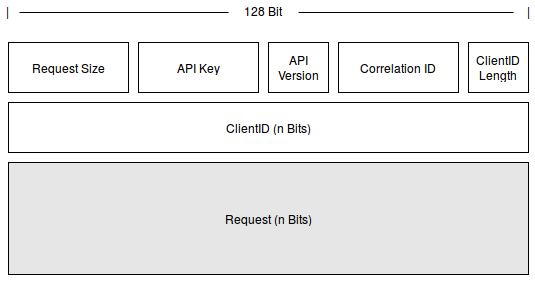
\includegraphics[width=0.7\textwidth]{images/protocol-request-header.png}
    \caption{Common Request Header}
    \label{fig:protocol-request-header.png}
\end{figure}

\begin{figure}[H]
    \centering
    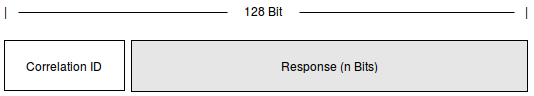
\includegraphics[width=0.7\textwidth]{images/protocol-response-header.png}
    \caption{Common Request Header}
    \label{fig:protocol-response-header.png}
\end{figure}

\subsection{Metadata API}
Describes the currently available brokers, their host and port information, and
gives information about which broker hosts which partitions.

\textbf{Not implemented yet}

\subsection{Produce API}
Send messages to the broker.

\textbf{Not implemented yet}

\subsection{Fetch API}
Fetchs / Consumes messages from the broker.
\subsection{Offset API}
Get information about the available offsets for a given topic partition

\textbf{Not implemented yet}

\subsection{Offset Commit API}
Commit a set of offsets for a consumer group

\textbf{Not implemented yet}

\subsection{Offset Commit API}
Fetch a set of offsets for a consumer group

\textbf{Not implemented yet}

\subsection{Types}

The design of the Apache Kafka protocol allows to make a distinction between three kind of types:
\begin{enumerate}
  \item Related to request
  \item Related to response
  \item Related to data (for either request or response but can also be used for the \fnurl{Apache Kafka Log}{http://kafka.apache.org/documentation.html\#log} component since log files (on-disk) hold the same structure)
\end{enumerate}

As for request and response related types we had to introduce an own naming
convention. As a matter of fact, not every field of some kind of request or
response will be unique. For more than once, there is a field that will
represent a \textit{topicName} for example. Thus, naming the field \textit{
topicName} would have been the obvious solution but since the record syntax in
Haskell won't allow to use the same name for a field twice - even in different
data types - we defined unique prefixes for each request and response as being
listed in the following table:

\begin{table}[h]
\centering
\begin{tabular}{|l|l|l|}
\hline
\textbf{API}            & \textbf{Request (Rq)} & \textbf{Response (Rs)} \\ \hline
Metadata API (Md)       & MetadataRequest       & MetadataResponse       \\ \hline
Produce API (Pr)        & ProduceRequest        & ProduceResponse        \\ \hline
Fetch API (Ft)          & FetchRequest          & FetchResponse          \\ \hline
Offset API (Of)         & OffsetRequest         & OffsetResponse         \\ \hline
Offset Commit API (Ofc) & OffsetCommitRequest   & OffsetCommitResponse   \\ \hline
Offset Fetch API (Oft)  & OffsetFetchRequest    & OffsetFetchResponse    \\ \hline
\end{tabular}
\end{table}

As mentioned before, the representation of the protocol structure is
implemented using the Haskell \fnurl{type
system}{https://wiki.haskell.org/Type}, more concrete using data types created
for our need using the named fields - also known as \fnurl{record
syntax}{http://en.wikibooks.org/wiki/Haskell/More_on_datatypes}.

Given this, a further step of abstraction is introduced by creating types for
the binary representation of a protocol field. The actual type for the data
fields in the protocol have to match an unsigned integer type of its length.
This can easily be done using the
\fnurl{Data.Word}{http://hackage.haskell.org/package/base-4.7.0.2/docs/Data-Word.html}
library. However, while repetitive writing \textit{WordX} (where is stands for
8-, 16-, 32-, or 64 bit) is rather intuitive, creating aliases using the
\textit{type} keyword will result in better readable code, as well as structure
of the implemented protocol.

As a result, a typical data type is described as follows, while details are
hidden for demonstration purposes.:

\begin{lstlisting}
-- more
data Partition =
    ----------------------
    -- ProduceRequest (pr)
    ----------------------
    RqPrPartition
    { rqPrPartitionNumber :: !PartitionNumber
    , rqPrMessageSetSize  :: !MessageSetSize
    , rqPrMessageSet      :: [MessageSet]
    }
    |
    ----------------------
    -- FetchRequest (ft)
    ----------------------
    RqFtPartition
    { rqFtPartitionNumber :: !PartitionNumber
    , rqFtFetchOffset     :: !Offset
    , rqFtMaxBytes        :: !MaxBytes
    }
    |
-- more
\end{lstlisting}

\section{Subsystems}

\subsection{Channeling}

The
\fnurl{Control.Concurrent.Chan}{http://hackage.haskell.org/package/base-4.8.0.0/docs/Control-Concurrent-Chan.html}
package provides a one-way FIFO communication channel. In
our case, this concept is being used to separate the
three mentioned subsystems from each other. The fact that
\textit{chan} is unbounded brings a risk. While
\textit{writeChan} -- which is being used to write to a
channel -- succeeds immediately, there is a chance that the
consuming thread is not able to read the same amount of
data in a given time and thus the channel will grow in
an unchecked manner. \cite{o2008real}

TODO: sanctions? do we have to block the producer for a short time?

TODO: tell why 2 separate channels are better than 1 two-way

\subsubsection{Request Channel (ReqChan)}

\subsubsection{Response Channel (ResChan)}


\subsection{Network Layer}

TODO: introduction to tasks of networking layer, then ref to socket server implementation

\subsection{API Layer}

TODO: introduction to tasks of api layer, then ref to request and error handling

\subsection{Log Subsystem}

TODO: introduction to tasks of log subsystem, then ref to persistance section


\section{Socket server implementation}

\begin{figure}[H]
    \centering
    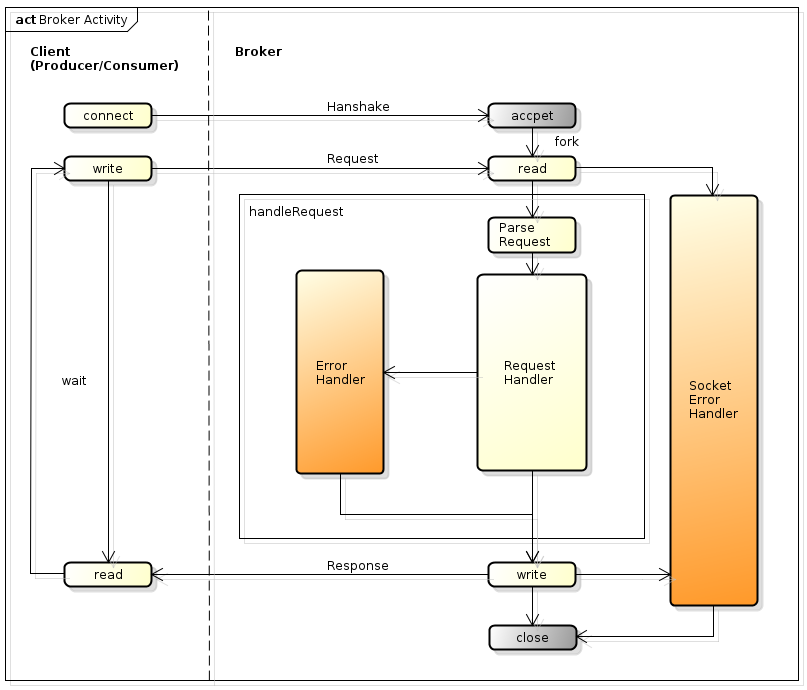
\includegraphics[width=0.7\textwidth]{images/broker-activity.png}
    \caption{Broker request handling concept}
    \label{fig:broker-activity.png}
\end{figure}

TODO: tell about Network.Socket

\section{Request Handling}

\begin{figure}[H]
    \centering
    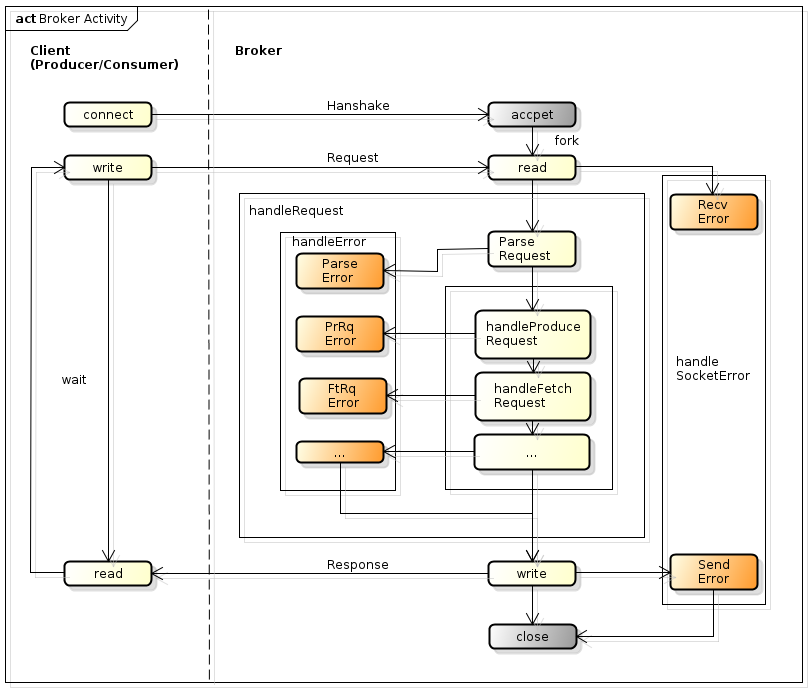
\includegraphics[width=0.7\textwidth]{images/broker-activity-detail.png}
    \caption{Broker request handling concept in detail}
    \label{fig:broker-activity-detail.png}
\end{figure}


\section{Error Handling}

\begin{figure}[H]
    \centering
    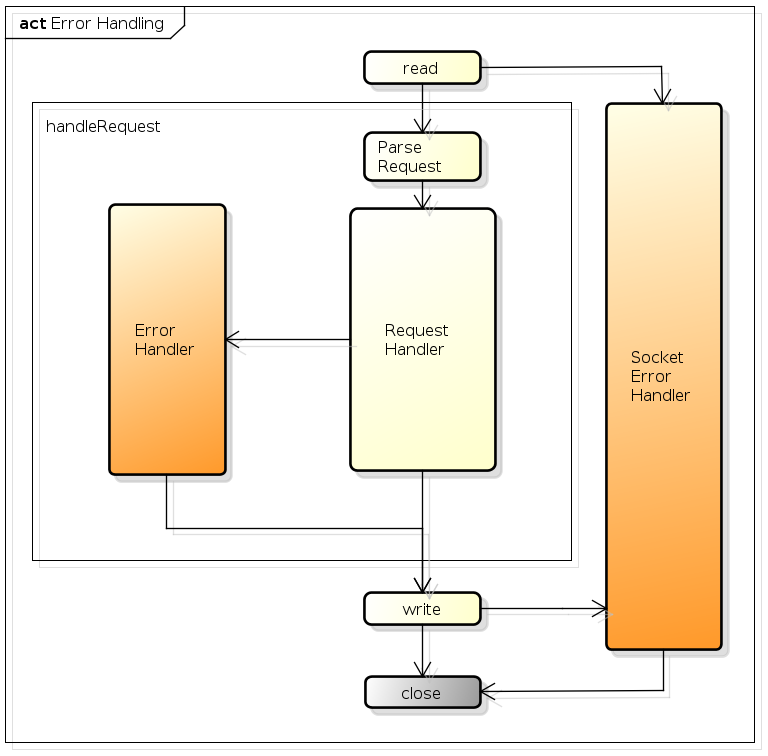
\includegraphics[width=0.7\textwidth]{images/broker-error-activity.png}
    \caption{Broker error handling concept}
    \label{fig:broker-error-activity.png}
\end{figure}


\begin{figure}[H]
    \centering
    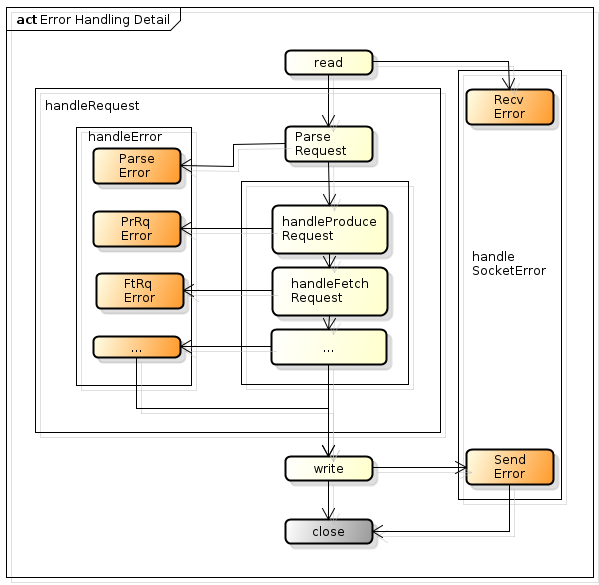
\includegraphics[width=0.7\textwidth]{images/broker-error-activity-detail.png}
    \caption{Broker handling concept in detail}
    \label{fig:broker-error-activity-detail.png}
\end{figure}

TODO: Either, Control.Monad.Error, Custom error types

\section{Persistence}

\subsection{Indexing}

\subsection{Storage Layout}

- for each topic a folder
- separate folders over partitions (1;2) -> topic\_0; topic\_1
- file name: offset of the first message it contains (next file: S bytes (max log size, given in configuration) from previous file)
- file format: sequence of log entries
- log entry: N (4 byte integer -> message length) followed by message (N message bytes)
- message: unique identifier (64 bit integer offset -> byte position of the start of this message in the stream of all messages ever sent to that topic on that partition)

On-disk format of a message:

offset: 8 bytes
message length : 4 bytes (value: 1+4+n) 
magic value  : 1 byte
crc            : 4 bytes
payload        : n bytes
    ?:              : 1 byte
    ?:              : 4 bytes
    message length  : 4 bytes
    message         : n bytes

\subsection{Read / Write}

\subsection{Optimization}

Next to optimizations like batching in the network layer \todo{ref to network},
we do also provide some optimizations in terms of I/O. \todo{Kafka: a
Distributed Messaging System for Log Processing}.

\subsubsection{Page Cache:}

First of all, We therefore avoid to explicitly cache messages in memory but
instead rely on the underlying file system cache. This has the benefit of
avoiding double buffering since messages are only cached in the page cache.
Thus, even if the broker process has to be restarted, the cache retains warm.

\todo{more details on modern os and page cache}

\subsubsection{Sequential I/O: }

While producers and consumers lead the broker to access
segments of files, the actual access which taking place is going to be a
sequential access rather than random. This will reduce seeking time to 1 per
partition. In fact, the broker holds a point on a given offset whereas all
messages below the pointer can be considered as already consumed and all
messages with offset greater than the provided one as unconsumed. Now since
messages are ordered this will lead to a sequential I/O with a constant seeking
time (O(1)).


\subsubsection{Internal data transfer:}

As mentioned earlier, HMB omit explicit caching but instead relies on the file system.
Keep this in mind, the actual network access for consumers can be optimized as well.
While a typical approach to sending bytes from a local file to a remote
socket involves the following steps: 
\begin{enumerate}
  \item Read data from storage (disk)
  \item Copy data from the page cache to an application buffer
  \item Copy application buffer to a kernel buffer
  \item Send kernel buffer to the socket
\end{enumerate}

With the help of the sendfile API \todo{ref} it is possible to 
transfer bytes from a file channel to a socket channel, whereas the delivery process will result in the following steps:

\begin{enumerate}
  \item Read data from storage (disk)
  \item Send data from page cache to the socket
\end{enumerate}


